\chapter{Background}\label{background}

\epigraph{The stars are not distant objects to be admired from afar. They are our partners in exploration and discovery, and we must learn to live and work with them if we are to achieve our goals.}{Arthur C. Clarke}

The evolution of a star in isolation, namely single star evolution, is predominantly determined by the stellar mass. Stars with $M \leq 2$ M$_{\odot}$, $2 < M \leq 8$ M$_{\odot}$ and $M > 8$ M$_{\odot}$ are classified as low-, intermediate-, and high-mass, respectively. In their attempt to achieve hydrostatic and thermal equilibrium, stars generate temperatures and pressures that allow for nuclear burning. The cycles of nuclear burning and fuel exhaustion regulate the evolution of a star and set the various phases during the stellar lifetime. These burning cycles can be viewed as long-lived, but transient disruptions to a star's (or at least its core's) inexorable shrinkage under the effect of gravity. The virial theorem dictates this contraction is caused by the fact that stars are hot and lose energy through radiation. 







\begin{comment}
 Despite the inherent rarity predicted by the initial mass function (IMF, see e.g. \cite{chabrier2005initial, dib2018emergence}), massive stars play a key role in the evolution of the Universe. They are the main source of UV radiation and heavy elements. They serve as a significant source of mixing and turbulence in the interstellar medium (ISM) of galaxies through a combination of winds, outflows, expanding HII regions, and supernova explosions. Galactic dynamos are powered by turbulence in conjunction with differential rotation. Cosmic rays are accelerated by the interaction of galactic magnetic fields and supernova shock fronts. The ISM is primarily heated by cosmic rays, UV radiation, and the dissipation of turbulence, whereas it is finally cooled by heavy metals present in dust, molecules, and in atomic/ionic form. Therefore, massive stars have a significant impact on galaxies' physical, chemical, and morphological structure \citep{kennicutt2005role}. However, the physical mechanisms behind the birth, development, and demise of massive stars remain elusive in comparison with low-mass stars \citep{zinnecker2007toward}. 
\end{comment}

\section{Timescales of stellar evolution}\label{sec:timescales}

The fundamental timescales of stellar evolution are the dynamical, thermal and nuclear timescales. The dynamical timescale is the characteristic time required for a star to collapse under its own gravitational force in the absence of internal pressure:
\begin{equation}\label{eq:dynamical_timsecale}
    t_{dyn} = \sqrt{\frac{R^3}{GM}} \sim 0.02 \left( \frac{R}{R_{\odot}} \right)^{3/2} \left( \frac{M}{M_{\odot}}\right)^{1/2} \; \text{days},
\end{equation}
where $R$ and $M$ are the star's radius and mass. It is a period on which a star might expand or contract if its hydrostatic equilibrium were disrupted, e.g. in case of sudden mass-loss.

Thermal (or Kelvin-Helmholtz) timescale indicates how quickly changes in a star's thermal structure may occur. It is therefore also the period on which a star responds when its thermal equilibrium is disturbed:
\begin{equation}\label{eq:thermal_timsecale}
    t_{th} = \frac{G M^2}{2RL} \sim 1.5 \times 10^7 \left( \frac{M}{M_{\odot}} \right)^{2} \frac{R_{\odot}}{R} \frac{L_{\odot}}{L} \; \text{yr},
\end{equation}
where L is the star's luminosity.

Finally, the nuclear timescale corresponds to the time required for the star to exhaust its nuclear fuel supply at its current luminosity: 
\begin{equation}\label{eq:nuclear_timsecale}
    t_{nuc} = \frac{\phi M_{nucl} c^2}{L} \sim 10^{10} \frac{M}{M_{\odot}} \frac{L_{\odot}}{L} \; \text{yr},
\end{equation}
where $\phi$ is the efficiency of nuclear energy production, $M_{nuc}$ is the amount of mass available as fuel, and $c$ is the light speed. For core hydrogen burning, $\phi = 0.007$ and $M_{nucl} \sim 0.1 M$ \citep{pols2011stellar}.

Typically $t_{nuc} >> t_{th} >> t_{dyn}$, while assuming a mass-luminosity relation of $L \propto M^{\alpha}$, with empirically $\alpha \sim 3-4$ \citep{eker2015main}, it follows that intermediate- and high-mass stars live shorter and evolve faster than low-mass stars.

%\subsection{Hertzsprung-Russell Diagram}\label{sub:HR_diagram}

\section{Evolution of intermediate-mass stars in isolation}\label{sec:single_star_evolution}

\begin{comment}

The late stages of their evolution, namely the Asymptotic Giant Branch (AGB) phase, is characterized by rich nucleosynthesis and strong mass loss, that eventually removes their envelopes, leaving behind a degenerate C-O core as the central star of a planetary nebula\citep{pols2011stellar}. Additionally, the lost mass provides material for future generations of stars, 
\end{comment}


The \ac{hrd} diagram is a useful tool for studying stellar evolution. It is a logarithmic representation of the surface luminosity (or absolute magnitude) of a star as a function of its effective temperature (or spectral type). Furthermore, it is divided into five different regions, namely the \ac{ms}, the \ac{rgb}, the horizontal-giant branch, the \ac{agb} and the region of degenerate stars. A star, depending on its mass, will pass through some of these regions during its lifetime as a result of the interplay between nuclear reactions and gravitational contraction. 

\begin{figure}[H]
    \centering
    \includegraphics[width=0.9\textwidth]{Thesis/graphs/HR_inter_stars.pdf}
    \caption{Hertzsprung-Russell diagram. Evolutionary tracks for three stars with masses 3, 5.5 and 8 M$_{\odot}$ at solar metallicity until the end of Helium burning. Specific moments in the evolution of the stars are noted by black circles and squares as explained in the text. I calculate the tracks using MESA \citep{paxton2010modules,paxton2013modules,paxton2015modules,paxton2019modules}. The dashed lines show lines of constant radii by means of the Stefan–Boltzmann law.}
    \label{fig:HR_inter_stars}
\end{figure}
Intermediate-mass stars have a complex evolutionary path that includes multiple phases of fusion and contraction. The \ac{hrd} diagram in \cref{fig:HR_inter_stars} shows three evolutionary tracks for intermediate-mass stars. From left to right, the black circles correspond to the \ac{zams} and \ac{tams}. At \ac{zams}, the star having started the hydrogen burning in its core, achieves \ac{te}, $L_{nuc}/L =1$, while \ac{tams} is defined as the core hydrogen exhaustion point. Additionally, the black squares represent the start and end of helium burning in the core, respectively.
\ac{tams} and the end of helium burning in the core are both defined as the point at which the hydrogen and helium core mass fractions are $< 0.01$, respectively. The change in the star's physical radius occurs on different timescales depending on the physical mechanism buried beneath these processes. On nuclear timescale, see \cref{eq:nuclear_timsecale}), stars evolve throughout the \ac{ms} and the helium-burning phase, while on thermal timescale (see  \cref{eq:thermal_timsecale}), stars expand during the H-shell burning phase.
\begin{figure}[H]
    \centering
    \includegraphics[width=0.9\textwidth]{Thesis/graphs/HR_evolution.pdf}
    \caption{Evolution of 5.5 M$_{\odot}$ at solar metallicity until a the end of the early \ac{agb} phase. The evolutionary phases are categorized in different colors as explained in the text. I calculate the tracks using MESA \citep{paxton2010modules,paxton2013modules,paxton2015modules,paxton2019modules}. The dashed lines show lines of constant radii by means of the Stefan–Boltzmann law.}
    \label{fig:HR_evolution}
\end{figure}
\cref{fig:HR_evolution} illustrates the evolution of a 5.5 M$_{\odot}$ star in isolation from the beginning of the \ac{ms} until the end of the early \ac{agb} phase. The evolutionary track is further categorized into sections and subsections: 
\begin{enumerate}
    \item Main-Sequence (green)
    \item Giant branch: 
        \subitem Hertzsprung gap or subgiant branch (yellow) 
        \subitem Red giant branch (red)
    \item Blue loop (blue)
    \item Asymptotic giant branch (black)
\end{enumerate}
During \ac{ms}, hydrogen is fused into $^4$He. Independent of the ongoing reaction channel (pp or CNO), the luminosity of the star increases during this phase, (L$\,\propto\,\mu^{4}\,M^3$), due to the change in the core's composition ($\mu$ increases). Nevertheless, the way in which a star evolves through the \ac{ms}-phase depends on its mass. Intermediate-mass stars have masses M\,$\geq$\,1.3\,M$_\odot$ and are driven by the CNO-cycle ($\epsilon_{CNO}\,\propto\,\rho_{c}T^{18}_{c}$). The thermostatic action of the CNO-cycle causes the envelope to expand and, as a result, a decrease in effective temperature. In general, stars driven by the CNO-cycle evolve through larger radii and lower T$_{eff}$ than stars driven by the pp-cycle (low-mass stars). Additionally, intermediate-mass stars have convective cores, since the energy produced is too large to be transported by radiation ($\nabla_{rad} > \nabla_{ad}$). One effect of the convection on the evolution is that the \ac{ms}-lifetime is extended (more detailed discussion in \cref{sec:convection}). Another effect is that as the core approaches the end of H-burning, the reactions suddenly cease in the whole core, threatening the thermal equilibrium of the star. In response the temperature of the core needs to increase in order to keep the same energy generation rate leading to the contraction of the star. This is evident in the second part of the \ac{ms} (see \cref{fig:HR_evolution}), where we observe the ``hook'' feature. 

At \ac{tams}, when the hydrogen in the core has been depleted, hydrogen burning occurs in a shell around it, while the central temperature is insufficient to initiate He-burning. From that point on, the evolution is driven by the mirror principle and stars evolve towards red giants \citep{pols2011stellar}. The core contracts on $t_{th}$ in an attempt to reach \ac{te}, while the envelope expands. The aforementioned behavior is evident in \cref{fig:HR_inter_stars} and \cref{fig:HR_evolution}, as stars move towards bigger radii and lower effective temperatures. Intermediate-mass stars reach effective temperatures as low as 5000K ($\sim 10^{3.7}$K) before helium ignition. At this moment, they begin to ascend the \ac{rgb}, which is accompanied by a significant rise in luminosity and radius. Due to the low effective temperature the opacity of the envelope rises and the latter becomes gradually convective ($\nabla_{rad} \propto \frac{\kappa}{T^4}$, more detailed discussion in \cref{sec:convection}). The prohibited zone of the HR-diagram is located to the right of the \ac{rgb}, where hydrostatic equilibrium cannot be established. Any star in this zone will travel quickly towards the \ac{rgb}. The red giant star has a compact core and an extensive envelope that extends hundreds of solar radii. 

When the temperature in the core exceeds $T_c \sim 10^8 K$, helium core burning begins. $^4$He fuses into a mixture of $^{12}$C and $^{16
}$O via the $triple- \alpha$ and $C+\alpha$ reactions, respectively \citep{pols2011stellar}. Helium ignition is thermally stable for intermediate-mass stars. The contraction of the core seizes, the envelope starts to shrink and the stellar radius decreases on $t_{nuc}$. As the star begins to descend the \ac{rgb}, the temperature in the envelope gradually rises. As a result, the envelope progressively shifts from convective to radiative. From the transition point on, the star enters the blue loop with a helium burning core, a hydrogen burning shell, a radiative envelope, and a gradually increasing effective temperature, see \cref{fig:HR_evolution}.  Hence, the luminosity starts to rise, because it has a stronger dependence on the effective temperature than on the radius ($L \propto R^2 T_{eff}^4$). After the point where star reaches local maximum temperature, see \cref{fig:HR_evolution}, the evolution is similar with the second part of the \ac{ms} (``hook'' feature). Due to the convective core, the He-burning reactions suddenly cease in the whole core and not gradually. The temperature of the core ($T_c$) needs to increase in order to keep the same energy generation rate thus the pressure exerted on the core by the layers between the hydrogen burning shell and the core must also increase. This result to the decrease of the pressure that is exerted by these layers towards the hydrogen burning shell. Due to the thermostatic behavior of the CNO-cycle the pressure by the envelope towards the hydrogen burning shell must also decrease. This leads to the envelope's expansion and the reduction of the effective temperature until the end of He-burning, see Fig. \ref{fig:HR_evolution}.

The end of He-burning marks the beginning of the \ac{agb} phase (black part of the track in Fig. \ref{fig:HR_evolution}). This is a brief yet very important evolutionary phase of intermediate-mass stars. It is characterized by rich nucleosynthesis and the enrichment of the outer layers with heavy elements. More specifically, for stars with $M \geq 4M_{\odot}$, the convective envelope can penetrate down into the helium rich layers, dredging up He- and N-rich material. The late \ac{agb} phase is characterized by strong mass loss, that eventually removes the stellar envelopes, leaving behind a degenerate C-O core as the central star of a planetary nebula\citep{pols2011stellar}. Hence understanding the nature and history of intermediate-mass stars is critical for investigating chemical enrichment and energy generation in galaxies, as well as forecasting the fate of stars like our Sun. For a more in depth description of the \ac{ms} and post-\ac{ms} evolution, I direct the reader to \cite{pols2011stellar}.

\subsection{Stellar winds}\label{sub:winds}

Stellar winds play an important role in stellar evolution because they cause mass and angular momentum loss from stars. Even though they are fundamental in understanding the formation and evolution of stars, the stellar wind mechanisms involved are not well understood in many cases. Hence, $\dot{M}$ is frequently quite uncertain introducing significant complexities in the evolution of stars. Driven by observations and theoretical models, stellar winds are usually categorized in hot and cold winds, because they are generated by different mechanisms. Numerous mass-loss rate prescriptions have been proposed, with $\dot{M}$ varying in different parts of the HR diagram.

Hot, luminous stars (mostly OB-type \ac{ms} stars and blue supergiants) experience a stellar wind driven by radiation. Radiation pressure causes an outward acceleration at frequencies corresponding to absorption lines in the spectrum, where the interaction between photons and matter is strong. Because it is primarily the lines of the heavier elements that contribute to line driving, radiation-driven mass-loss is dependent also on metallicity \citep{vink2001mass}. Mass loss due to hot winds is relatively unimportant for intermediate-mass stars.

Cool, luminous \ac{rsg} produce a stellar wind, which is likely caused by a combination of stellar pulsations and radiation pressure on dust particles that accumulate in the cool outer atmosphere. Because there are no theoretical predictions, empirical formulas that fit the average observed mass-loss rates of stars of roughly solar metallicity are used in theoretical studies. For example, Reimers' mass-loss empirical formula \citep{reimers1975circumstellar} is commonly used to model the mass-loss on the \ac{rgb}:
\begin{equation}\label{eq:reimer}
    \dot{M}_{R} = -4 \times 10^{-13} \eta 
    \frac{L}{L_{\odot}}  \frac{R}{R_{\odot}} \frac{M_{\odot}}{M},
    \text{ M${\odot} \; yr^{-1}$},
\end{equation}
where $\eta$ is parameter of the order of unity.

During the final stages of evolution on the \ac{agb}, low- and intermediate-mass stars' outer atmospheres are cool enough that dust formation becomes significant enough to dominate the opacity. Such stars experience significant mass-loss, which removes the remaining envelope, leaving only a C-O \ac{wd} as their final remnant \citep{marigo2007evolution, pols2011stellar}. Blocker's mass-loss empirical formula \citep{bloecker1995stellarI,bloecker1995stellarII} is commonly used to model the mass-loss on the \ac{agb}:
\begin{equation}\label{eq:blocker}
    \dot{M}_{Bl} = -4.83 \times 10^{-9} M^{-2.1} L^{2.7} \dot{M}_{R},
    \text{ M${\odot} \; yr^{-1}$}.
\end{equation}

Other mass-loss prescriptions that are common in theoretical studies are given by \cite{de1988mass,nieuwenhuijzen1990parametrization}. The high mass-loss rate during the \ac{agb} phase defines both the maximum luminosity that a low- or intermediate-mass star may achieve on the \ac{agb}, and its ultimate mass, i.e. the mass of the \ac{wd} remnant.

\begin{comment}

On the other hand, for masses greater than 15 M$_{\odot}$, mass-loss by stellar winds becomes important during all evolution phases, including the main sequence. Observations in the ultraviolet and infrared spectrum show that these luminous massive stars experience rapid mass outflows (stellar winds) that can gradually erode their outer layers. For masses greater than 30 M$_{\odot}$, the mass-loss rates, $\dot{M}$, are so great that the mass-loss timescale, $t_{ml} = M / \dot{M}$, becomes shorter than the nuclear timescale, $t_{nuc}$.
\end{comment}

\subsection{Convection}\label{sec:convection}

A variety of internal mixing process can impact the life cycle of stars. Apart from convection, convective overshooting, semi-convection, and rotationally induced mixing are the most important internal mixing process \citep{schootemeijer2019constraining} and are still poorly understood. In this work, semi-convection and rotationally induced mixing are not taken into account as these are expected to be more important for massive stars ($M>8$ M$_{\odot}$) \citep{langer2012presupernova}. However, convection and convective overshooting are being explored.

\begin{comment}
    
I investigate the role of convective overshooting, which proved to be mostly important for the inner high-density regions of the star. Convection, on the other hand, proved to play an important role in the construction of the hydrodynamical models (see \cref{sec:1D_to_3D}).
\end{comment}

Nuclear reactions at a star's core generate energy,
which is transported to the stellar surface, on roughly thermal timescale, see \cref{eq:thermal_timsecale}, preserving the \ac{te} of the star. As a result, an energy density gradient exists, resulting in a net energy flux towards the stellar surface. Since an energy density gradient is associated with a temperature gradient, the more the luminosity to be transported, the greater the temperature gradient required. However, there is an upper limit to the temperature gradient inside a star; This limit is called adiabatic temperature gradient,
\begin{equation}\label{eq:ad_tempe_grad}
    \nabla_{ad} = \left ( \frac{d logT}{d logP} \right)_{ad},
\end{equation}
and describes the logarithmic variation of temperature under adiabatic compression or expansion. An adiabatic process occurs on such a short (dynamical) timescale that there is no heat exchange with the environment.

In the case that the temperature gradient limit is surpassed, gas instability, called convection, occurs \citep{pols2011stellar}. Convection refers to the collective (bulk) cyclic movements of gas particles. This is a key activity in stellar interiors because it not only effectively transports energy, but also results in fast mixing. Another important aspect of convection is that the energy transportation and mixing occur on local dynamical timescale $t_{conv}$, where $t_{conv} << t_{th}$. This means that, while convection can efficiently transfer a large amount of energy, it does so at a nearly constant temperature $T$, indicating that the process is nearly adiabatic. Unfortunately though, it remains one of the least known aspects of stellar physics.

For such an adiabatic process the equation of state can be approximated by a polytropic relation
\begin{equation}\label{eq:adiabatic_eos}
    P \propto \rho^{\gamma_{ad}}.
\end{equation}
\cref{eq:adiabatic_eos} is of great importance. The absence of $T$ implies that the mechanical structure of convective stars or convective stellar envelopes is independent of the stellar temperature, (see \ac{rgb} in \cref{fig:HR_evolution}). For an ideal gas, ${\gamma_{ad}} = 5/3$ and/or $\nabla_{ad} = 0.4$ \citep{pols2011stellar}.

\begin{comment}
Another important consequence of \cref{eq:adiabatic_eos} is
\begin{equation}\label{}
    R \propto M^{-1/3}
\end{equation}
which derives by combining \cref{eq:adiabatic_eos} with the equations of 

It corresponds to a polytrope of $n = \frac{3}{2}$, where $\gamma_{ad} = 1+ \frac{1}{n}$ and 

From \cref{eq:ad_tempe_grad} one can see that the temperature stratification of a convective star can be described by a power law $T \propto P^{\nabla_{ad}}$.  Additionally, for an ideal gas, $P \propto \rho T$ and by combining the above one can easily see that

where $\gamma_{ad} = \frac{1}{1-\nabla_{ad}}$.
\end{comment}



{\bf Stability against convection}


Assuming that photons alone carry the produced energy, the dimensionless radiative temperature gradient is defined as
\begin{equation}\label{eq:radia_tempe_grad}
    \nabla_{rad} = \left ( \frac{d logT}{d logP} \right)_{rad} = \frac{3}{16 \pi \alpha c G} \frac{\kappa l P}{m T^4},
\end{equation}
where $\alpha$ is the radiation constant, $c$ the speed of light and $G$ the gravitational constant. The variable $l$ is the local luminosity, $\kappa$ the Rosseland mean opacity and $m$ the mass coordinate.  \cref{eq:radia_tempe_grad} describes the logarithmic variation of temperature with pressure, which represents the depth, for a star in \ac{he} if energy is transported only by radiation.

Using \cref{eq:ad_tempe_grad}, \cref{eq:radia_tempe_grad} and assuming ideal gas, I present the Ledoux criterion,  which states that a stellar layer is stable against convection if:
\begin{equation}\label{eq:Ledoux_criterion}
    \nabla_{rad} < \nabla_{rad} +  \nabla_{\mu},
\end{equation}
where $\nabla_{\mu}$ is the gradient of the mean molecular weight through the star. Because nuclear processes create more and more heavy elements in deeper layers, the mean molecular weight generally increases inwards. Typically, $\nabla_{\mu} \geq 0$, indicating that a composition gradient has a stabilizing effect.

For chemically homogeneous layers, the stability criterion against convection reduces to the Schwarzwild criterion:
\begin{equation}\label{eq:Schwarzwild_criterion}
    \nabla_{rad} < \nabla_{ad}.
\end{equation}
 

{\bf Convection occurrence}

Using \cref{eq:radia_tempe_grad} and the Schwarzwild criterion, \cref{eq:Schwarzwild_criterion}, convection occurs:
\begin{itemize}
    \item In opaque regions of the star, meaning $\kappa$ is large. Since the opacity increases with decreasing temperature \citep{pols2011stellar}, I expect the envelopes of cool star to be convective. For example, low-mass or intermediate-mass stars during the \ac{rgb} and \ac{agb} phase, see \cref{fig:HR_inter_stars} and \cref{fig:HR_evolution}.
    \item In regions of the star with large energy flux, meaning $\frac{l}{m}$ is large. For example, the cores of intermediate- and high-mass stars, where nuclear reactions are driven by the CNO-cycle ($\epsilon_{CNO} \propto \rho_c T_{c}^{18})$.
\end{itemize}

{\bf Convective overshooting}

Convective overshooting refers to the process of mixing beyond the boundaries of convective regions, which can occur when convective cells penetrate into radiative regions due to their non-zero velocity \citep{alongi1993evolutionary,brott2011rotating,schootemeijer2019constraining}. In stars with convective cores, e.g. intermediate- and high-mass stars, the size of the core is effectively enlarged through mechanisms such as convective core overshooting. This overshooting brings additional hydrogen into the core and therefore directly impacts the final He-core mass, while extents the \ac{ms} lifetime and affects the post-\ac{ms} evolution.

The extent of the overshooting region is not known reliably from theory. However, in stellar evolution calculations, overshooting is usually treated based on \cite{herwig2000evolution}. The latter investigate in detail the impact of overshooting on the evolution of \ac{agb} stars. Based on their model the extended mixing is treated time-dependently, and the efficiency decreases exponentially as the geometric distance from the convective boundary increases. 



\section{Binary star systems}\label{sec:binary_evolution}

The evolution of a star in isolation could be summarized as:

{\it Stars contract because they are hot and lose energy through radiation (Virial Theorem), while nuclear burning cycles serve as long-lived but transitory interruptions to a star's (or at least its core's) inevitable contraction due to gravity}. 

Despite that seemingly straightforward picture, stars tend to form in multiple systems (see \cref{fig:stellar_companions}). Binaries particularly, which consist of two stars that orbit around a shared center of mass and are gravitationally connected to each other, are of immense importance. By nature, they reveal more about themselves, particularly their masses and diameters, than other astronomical objects. This is especially true for eclipsing binaries \citep{prvsa2016physics}, which provide us with direct knowledge regarding spatial relations inside the source. Furthermore, close binaries are unique cosmic laboratories providing useful insights regarding different physical process. For example, gravitational wave emission is widely studied in binary mergers where both stars are compact objects \citep{cutler1994gravitational,abbott2017gw170608,abbott2019gwtc}, accretion as a power source in X-ray binaries \citep{lewin1997x,reig2011x}, while stellar interactions such as mass transfer, angular momentum exchange and tidal friction in close binaries. 


Despite the additional complexity that these stellar interactions provide to the evolution of these systems, they offer the necessary base for discussing stellar interactions in triple systems.  There are two fundamental reasons why may binaries transfer matter:

\begin{enumerate}
    \item During its evolution, one of the stars in a binary system may expand in radius (R$_{\star}$) or contract in binary separation (${\alpha}$) to the point where the companion's gravitational force can remove the outer layers of its envelope (Roche lobe overflow, RLOF).
    \item At some point in its evolution, usually during the late post-main-sequence phase, one of the stars may release most of its mass in the form of a stellar wind; part of this material will be gravitationally trapped by the companion (stellar wind accretion). 
\end{enumerate}

This section is mainly focused on interacting binaries via RLOF, (1). 

\subsection{The relative orbit}

The problem of describing the motion of two point masses
under the effect of their mutual gravity, namely the famous two-body problem, has been studied extensively and a derivation of the equations of motion is out of the project's scope. For a detailed review of the two body problem, I redirect the reader to  \cite{postnov2014evolution}. Nevertheless, based on the relative orbit model, two mutually interacting bodies' equations of motion can be simplified to a single equation representing the motion of one body in a reference frame centered on the other body. The moving body therefore behaves as if its mass was
\begin{equation}\label{eq:reduced_mass}
    \mu= \frac{M_1 M_2}{M_1 + M_2},
\end{equation}
which is known as the reduced mass. As a result, the evolution of binaries can be described by the stellar masses, $M_1$ and $M_2$, the semi-major axis, $\alpha$, and the eccentricity, $e$, of the relative orbit \citep{sana2012binary,postnov2014evolution,toonen2014popcorn}. It is worth noting that the orbital separation, is linked to the eclipse's semi-major axis, although they are not equal except in the case of a circular orbit. Additionally, $\alpha$ is commonly used in the literature to define both parameters. To avoid confusion, $r_{rel}$ refers the orbital separation of the binary components and $\alpha$ to the semi-major axis of the eclipse throughout this thesis.
\begin{figure}[H]
    \centering
    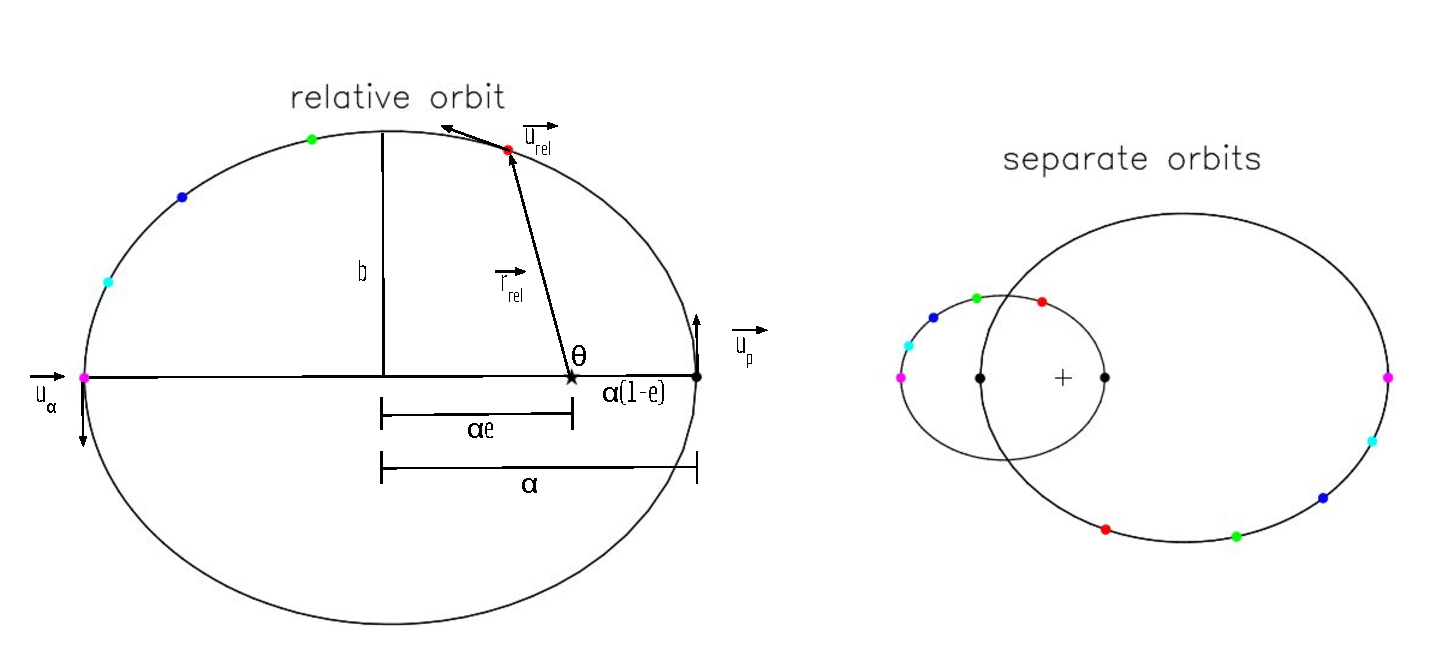
\includegraphics[width=0.9\textwidth]{Thesis/figures/relative_orbit.pdf}
    \caption{Relation between the relative orbit (left) and absolute orbits (right) of a
    binary, in this case Sirius. The black star symbol on the left figure represents the fixed star with the reference frame centered on it, while the circles represent the moving star with mass $\mu$. The absolute positions (right) are matched with the relative position of the moving body (left) via different colors.   The initial figure was taken by Frank Verbunt's lecture notes `Compact Binaries` and modified by me.}
    \label{fig:relative_orbit}
\end{figure}
The shape of the relative orbit is defined by the orbital energy and angular momentum per unit of reduced mass. For an elliptic relative orbit, specifically, the orbital energy per unit of reduced mass is
\begin{equation}\label{eq:orbital_energy}
    \epsilon = \frac{E}{\mu} = - \frac{G (M_1 + M_2)}{2\alpha}, \; \; \epsilon  < 0
\end{equation}
and the angular momentum per unit of reduced mass is
\begin{equation}\label{eq:orbital_ang_momentum}
    l = \frac{L}{\mu} = \vec{r_{rel}} \times \vec{u_{rel}} =\sqrt{G (M_1 + M_2) \alpha (1-e^2)}
\end{equation}
where $e$ is the eccentricity and $\alpha$ the semi-major axis of the eclipse, see \cref{fig:relative_orbit}. In the absence of mass loss, both $\epsilon$ and $l$ are constants of motion.  \cref{eq:orbital_energy} shows that the orbital energy is independent of the eccentricity, $e$ and in the elliptic case is always negative.

The relative position of the moving body, or the orbital separation of the binary components, see \cref{fig:relative_orbit}, is given as:
\begin{equation}\label{eq:relative_position}
    r_{rel} = \frac{\alpha (1-e^2)}{1+e \cos{\theta}}
\end{equation}
and its velocity as:
\begin{equation}\label{eq:relative_velocity}
    u_{rel}= \sqrt{GM \left( \frac{2}{r_{rel}} - \frac{1}{\alpha}\right)},
\end{equation}
where $M = M_1 + M_2$. Using \cref{eq:relative_velocity}, the semi-major axis is given as:
\begin{equation}\label{eq:semi-major_axis}
    \alpha = \frac{GM r_{rel}}{2GM - u_{rel}^2 r_{rel}}.
\end{equation}
Additionally, using  \cref{eq:orbital_ang_momentum} the eccentricity is given as:
\begin{equation}\label{eq:eccentricity}
    e = \sqrt{1 - \frac{|\vec{r_{rel}} \times \vec{u_{rel}}|^2}{G M \alpha}}.
\end{equation}

As a result, given the relative position and velocity of two stars, $M_1$ and $M_2$, the evolution of the binary can be describted using \cref{eq:orbital_energy}, \cref{eq:orbital_ang_momentum}, \cref{eq:semi-major_axis} and \cref{eq:eccentricity}.


\begin{comment}
For two stars of mass, $M_1$ at position $r_1$ and $M_2$ at position $r_2$, the the weighted mean position, namely the center of mass, can be defined as:
\begin{equation}\label{eq:center_of_mass}
    \vec{R_{cm}} = \frac{M_1 \vec{r_1} + M_2 \vec{r_2}}{M_1 + M_2}
\end{equation}
Furthermore, the reduced mass of the binary is defined as:
\begin{equation}
    \mu= \frac{M_1 M_2}{M_1 + M_2}
\end{equation}
\end{comment}


\subsection{Roche lobe overflow}\label{sub:roche_lobe}

The orbital parameters of the relative orbit are critical in defining the Roche model, a valuable tool in describing binary evolution. The Roche model describes the effective gravitational potential of the binary and it is based on three assumptions:
\begin{enumerate}
    \item The gravitational fields of both stars are assumed to be those of point masses.
    \item The binary orbit is assumed to be circular, $e=0$.
    \item The rotation of the stellar components is assumed to be synchronized with the orbital motion. 
\end{enumerate}
The Roche potential's crucial equipotential surface, which passes through the inner Lagrangian point $L_1$, defines two Roche lobes that encircle each star. Hence, each Roche lobe defines the volume in which material is gravitationally bound to the respective star. The Roche lobe can be approximated with accuracy better than $1\%$ by a sphere of radius $R_L$:
\begin{equation}\label{eq:roche_lobe}
    \frac{R_{L,1}}{\alpha} = \frac{0.49q^{2/3}}{0.6q^{2/3} + \ln{1+q^{1/3}}},
\end{equation}
where $q =M_1 / M_2$. $R_{L,2}$ is be given for $q =M_2 / M_1$. The Roche potential of a binary with $q=6.3/5.5 \approx 1.145$ and $\alpha = 1.24$ au is presented in \cref{fig:binary_equop}. The latter corresponds to the effective potential of $\xi$ Tau by replacing the inner binary masses, $M_1$ and $M_2$, with one star of mass $M = M_1 + M_2$.
\begin{figure}[H]
    \centering
    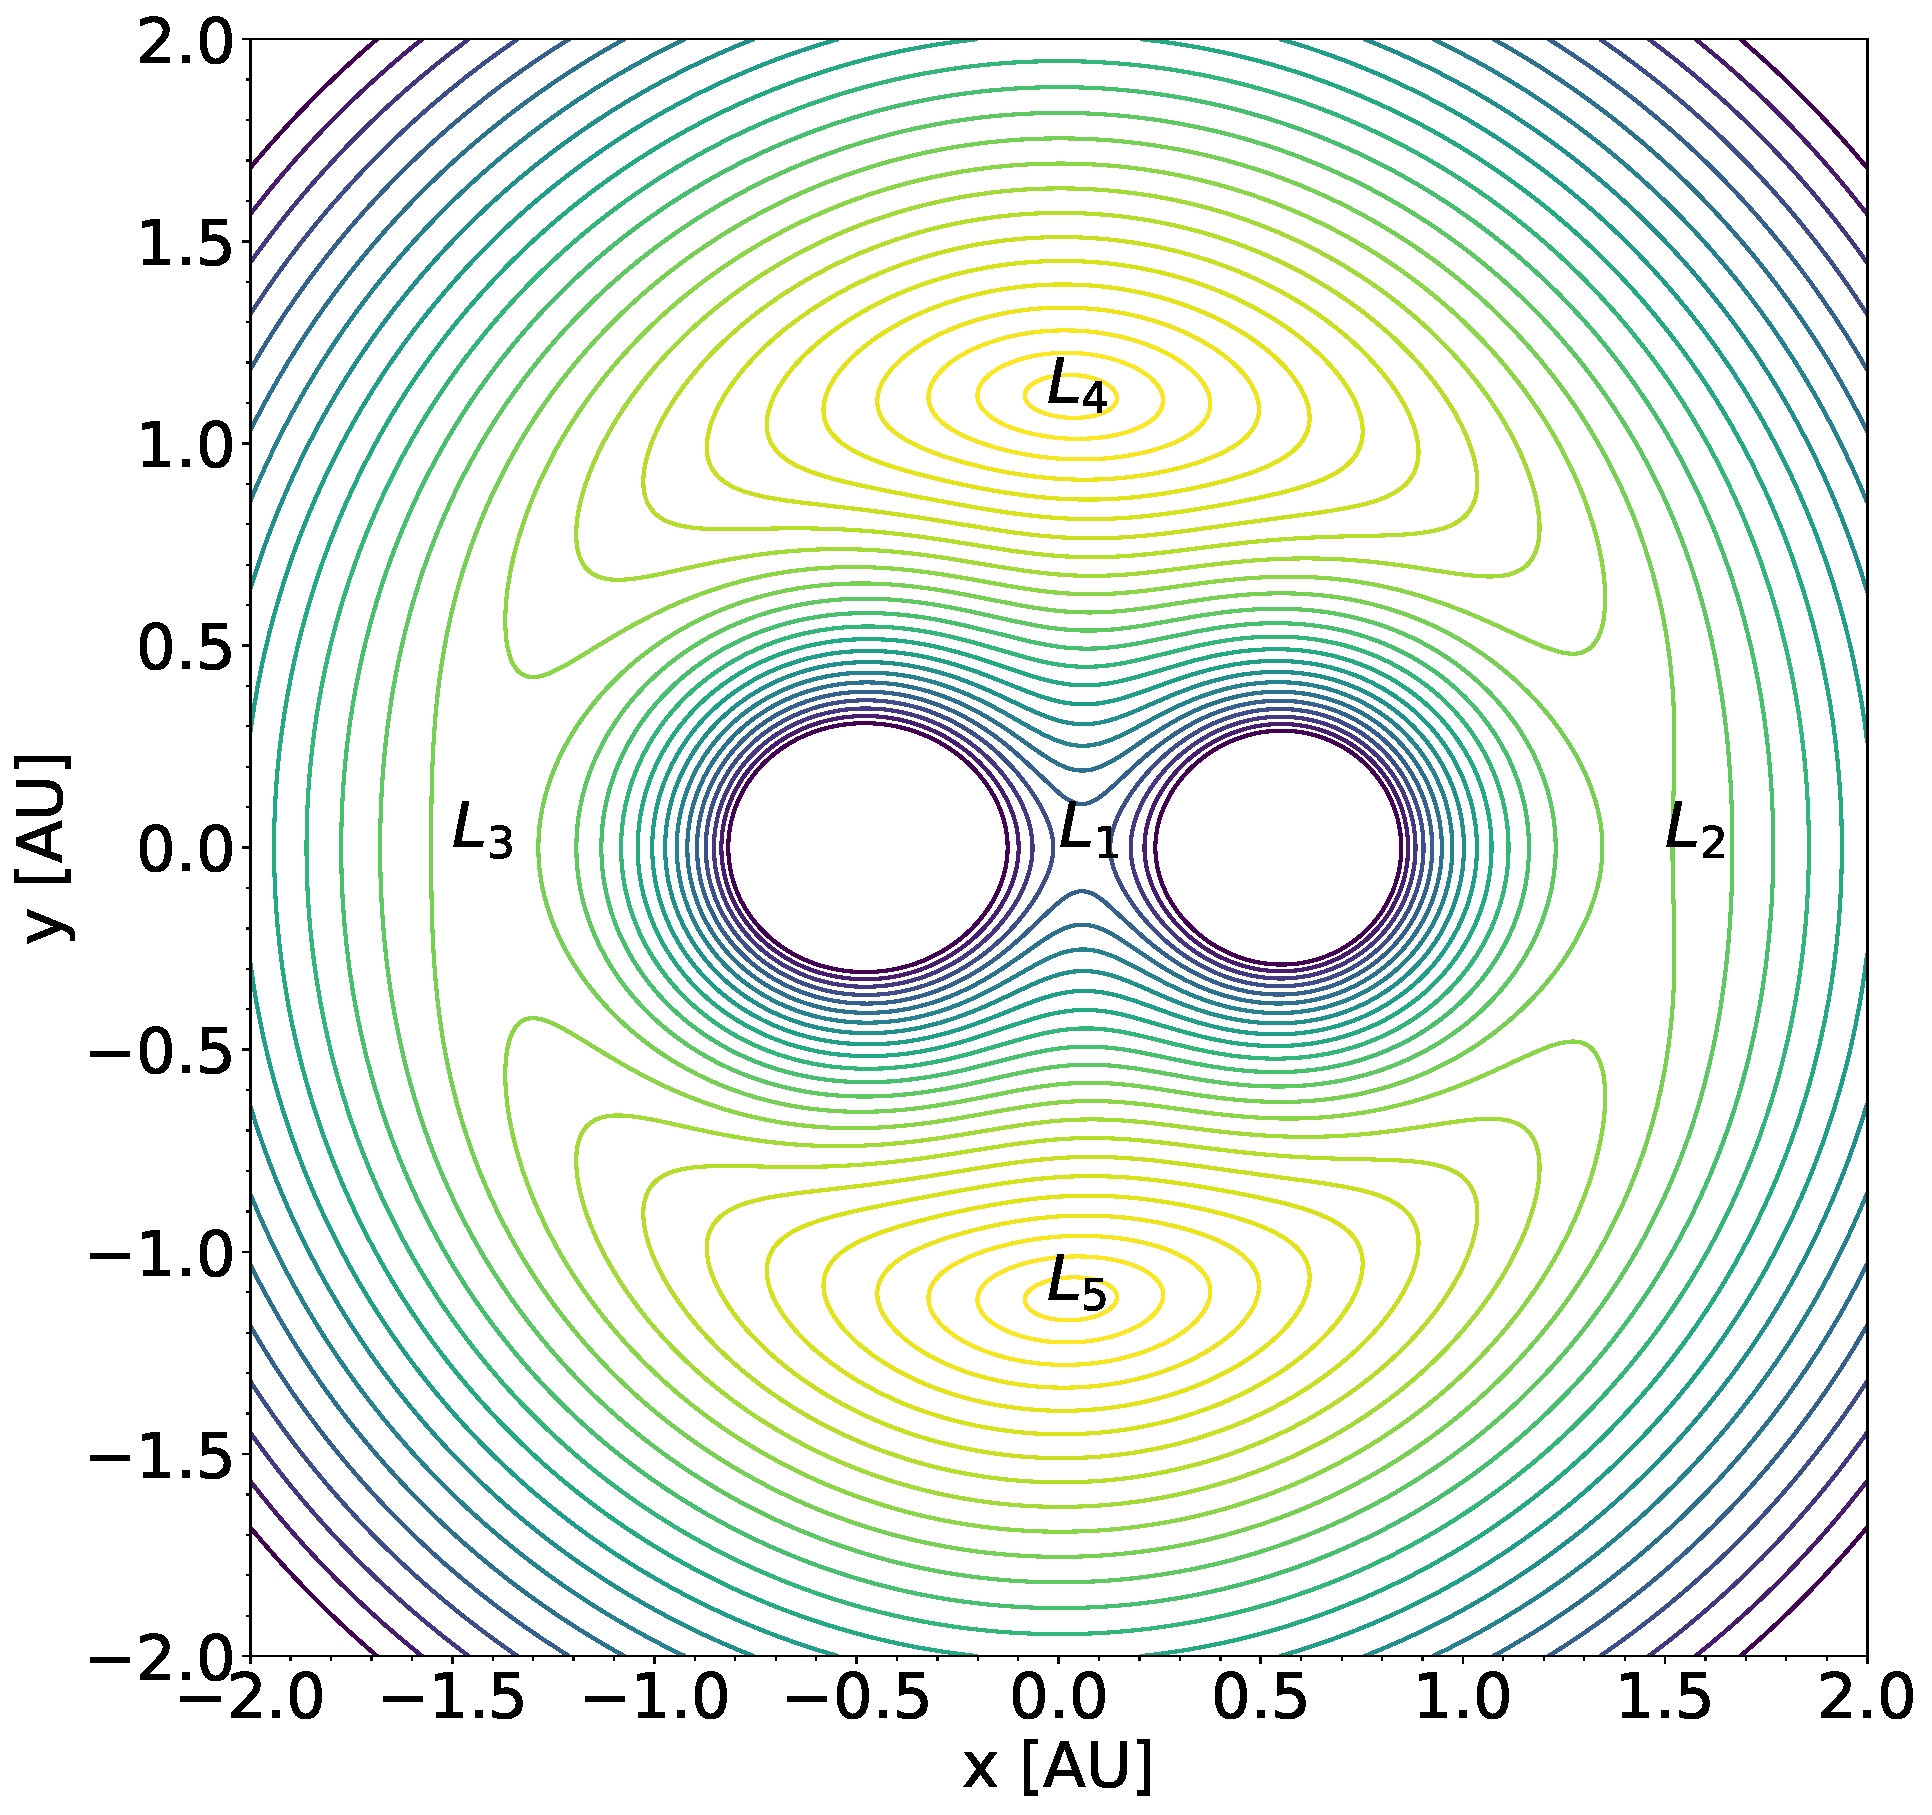
\includegraphics[width=0.9\textwidth]{Thesis/graphs/binary_equop.pdf}
    \caption{Contour plot of a binary's effective potential for $q=6.3/5.5 \approx 1.145$ and $\alpha = 1.24$ au. The five Lagrangian points are indicated as $L_1, L_2, L_3, L_4$ and $L_5$. I create the plot using the Hermite integrator which is part of AMUSE \citep{hut1995building}.}
    \label{fig:binary_equop}
\end{figure}
According to \cref{eq:roche_lobe}, the size of the Roche lobe is determined by the mass ratio $q$ and the orbital separation of the two stars, $\alpha$. The more massive star has a larger Roche lobe, whereas stars of equal mass have equal sized Roche lobes. Furthermore, the size of the Roche lobes is proportional to the orbital separation of the stars, so as the latter changes, so do the Roche lobes.

As discussed in \cref{sec:single_star_evolution}, stars contract and expand during their evolution. Additionally, the binary separation may decrease due to the loss of orbital angular momentum from the system via stellar wind mass-loss, see \cref{sub:winds} or gravitational radiation. As a result, the physical radius of a star, $R_{\star}$, may become larger than its Roche lobe radius, $R_{L}$. This scenario is called Roche-lobe overflow (RLOF) and matter from the outer layers of the Roche-lobe-filling star can freely move through the first Lagrangian point $L_1$ to the companion star. 


Mass flow via the $L_1$ point is a relatively complicated hydrodynamical problem, but the rate of mass transfer, $\dot{M}$, through $L_1$ is highly sensitive to the donor's fractional radius excess, $\frac{\Delta R}{R}$ . A comprehensive derivation of Bernoulli's law to the gas flow through the nozzle near $L_1$ results in 
\begin{equation}\label{eq:mass_loss_rate_anal}
    \dot{M} \propto \frac{M_{d}}{P} \left( \frac{\Delta R}{R}\right)^3,
\end{equation}
where $M_{d}$ is the donor mass and $P$ the orbital period of the binary.
\begin{comment}
    

Hence, the timescale of mass transfer is strongly dependent on the donor's fractional radius excess:
\begin{equation}\label{eq:mass_transfer_timescale}
   \frac{\Delta R}{R} \propto \frac{P}{t_{\dot{M}}}^{1/3}
\end{equation}
\end{comment}

According to \cref{sec:single_star_evolution}, intermediate-mass stars expand during MS on nuclear timescale and during RGB and AGB phases, on thermal timescale, see \cref{fig:HR_evolution}.  Hence, three cases of mass transfer can be distinguished:
\begin{enumerate}
    \item During the MS, namely Case A
    \item During post-MS and before helium exhaustion, namely Case B
    \item After helium exhaustion, namely Case C
\end{enumerate}
Considering that mass is the most important property for a star's evolution, see \cref{sec:single_star_evolution}, RLOF can significantly alter its evolutionary outcome. Thus, in a mass-transferring binary system, both stars are expected to deviate from the evolutionary paths they would have in the absence of mass transfer. 

\subsection{Orbital evolution during mass transfer}\label{sub:orbit_evol_mass_loss}

During mass transfer, the transferring matter carries angular momentum causing the orbital parameters of the relative orbit to change. By differentiating Eq. \eqref{eq:orbital_ang_momentum}, a general equation for the orbital evolution can be obtained:
\begin{equation}\label{eq:orb_ang_momen_derivative}
    2\frac{\dot{J}}{J} = \frac{\dot{\alpha}}{\alpha} + 2 \frac{\dot{M_1}}{M_1} + 2 \frac{\dot{M_2}}{M_2} - \frac{ \dot{M_1} + \dot{M_2}}{M_1 + M_2} - \frac{2e \dot{e}}{1-e^2},
\end{equation}
where the last term vanishes for circular orbits.

A basic assumption of \cref{eq:orb_ang_momen_derivative} is that the angular momentum stored in the rotation of the two stars is negligible compared to the orbital angular momentum. In most circumstances, this assumption is valid, however in the case of rapidly spinning objects, such as millisecond pulsars, the angular momentum contained in the pulsar's rotation may need to be considered.  

From \cref{eq:orb_ang_momen_derivative}, the evolution of the semi-major axis of the relative orbit during mass loss is given as:
\begin{equation}\label{eq:semimajor_axis_derivative}
     \frac{\dot{\alpha}}{\alpha} = 2\frac{\dot{J}}{J} - 2 \frac{\dot{M_1}}{M_1} - 2 \frac{\dot{M_2}}{M_2} + \frac{ \dot{M_1} + \dot{M_2}}{M_1 + M_2} + \frac{2e \dot{e}}{1-e^2},
\end{equation}
where the variable $\dot{J}$ represents angular momentum loss from the binary. 

The mass loss can be simply parameterized as
\begin{equation}\label{eq:mass_loss_non_cons}
    \dot{M_{a}} = - \beta \dot{M_{d}},
\end{equation}
where the subscript $a$ refers to the `accretor` and $d$ to the `donor`. In this case, $\beta$ is the fraction of the transferred mass that is accreted by the companion, and thus
\begin{equation}\label{eq:mass_loss_non_cons_2}
    \dot{M_{a}} + \dot{M_{d}} = (1-\beta) \dot{M_{d}}.
\end{equation}

In the ideal situation where all the transferred mass from the first star is accreted by the second, $\beta=1$, the orbital angular momentum of the binary is conserved, $\dot{J}=0$ and \cref{eq:semimajor_axis_derivative} reduces to
\begin{equation}\label{eq:orb_ang_momen_derivative_cons}
    \frac{\dot{\alpha}}{\alpha}= 2 \left( \frac{M_d}{M_a} - 1 \right) \frac{\dot{M_{d}}}{M_{d}} + \frac{2e \dot{e}}{1-e^2}.
\end{equation}    
This the case of conservative mass transfer and a close look to \cref{eq:orb_ang_momen_derivative_cons} reveals that for a circular orbit the orbital separation shrinks as long as $M_d > M_a$, while it expands when $M_d < M_a$. Finally, the minimum orbital distance is given for $M_d = M_a$. 

In the general case of RLOF, mass transfer is expected to be non-conservative meaning that  $\beta < 1$. Furthermore,
the ejected mass carries away orbital angular momentum from the system. The amount of specific angular momentum that is lost can be parameterized to be $\eta$ times the specific angular momentum of the binary:
\begin{equation}\label{eq:orb_ang_mom_non_cons}
    \frac{\dot{J}}{J} = \eta \frac{\dot{M_{a}} + \dot{M_{d}}}{M_{a} + M_{d}}.
\end{equation}
Using \cref{eq:mass_loss_non_cons_2} and \cref{eq:orb_ang_mom_non_cons}, \cref{eq:semimajor_axis_derivative} gives:
\begin{equation}\label{eq:orb_ang_momen_derivative_non_cons}
    \frac{\dot{\alpha}}{\alpha}= -2\frac{\dot{M_{d}}}{M_{d}} \left( 1- \beta\frac{M_d}{M_a} - (1-\beta)(\eta + \frac{1}{2}) \frac{M_d}{M_d + M_a}  \right)  + \frac{2e \dot{e}}{1-e^2}.
\end{equation}  
The parameters $\beta$ and $\eta$ are highly uncertain. Depending on the mass transfer mode, $\eta$ can be specified in terms of other quantities \citep{postnov2014evolution}.

Assuming circular orbit, $\beta$ and $\eta$ to be constants and by ignoring the internal angular momentum of the stars, \cite{portegies1995formation} shows that the evolution of the semi-major axis based on mass redistribution can be described as:
\begin{equation}\label{eq:semimajor_axis_no_cons}
    \frac{\alpha}{\alpha_{0}} = \left (\frac{M_{d} M_{a}}{M_{d,0} M_{a,0}} \right)^{-2} \left (\frac{M_{d} + M_{a}}{M_{d,0}+M_{a,0}} \right)^{2\eta +1},
\end{equation}    
where the `0` subscript corresponds to the initial values, before RLOF.
    






\section{Hierarchical triple star systems}\label{sec:triples_evolution}

The majority triple star systems are observed in hierarchical structures. More specifically, they consist of an inner binary and a distant star (hereafter tertiary/outer star) that orbits the center of mass of the inner binary system such as $\frac{\alpha_{in}}{\alpha_{out}} << 1$. A schematic of a hierarchical triple system is presented in \cref{fig:triple_schem}.
\begin{figure}[H]
    \centering
    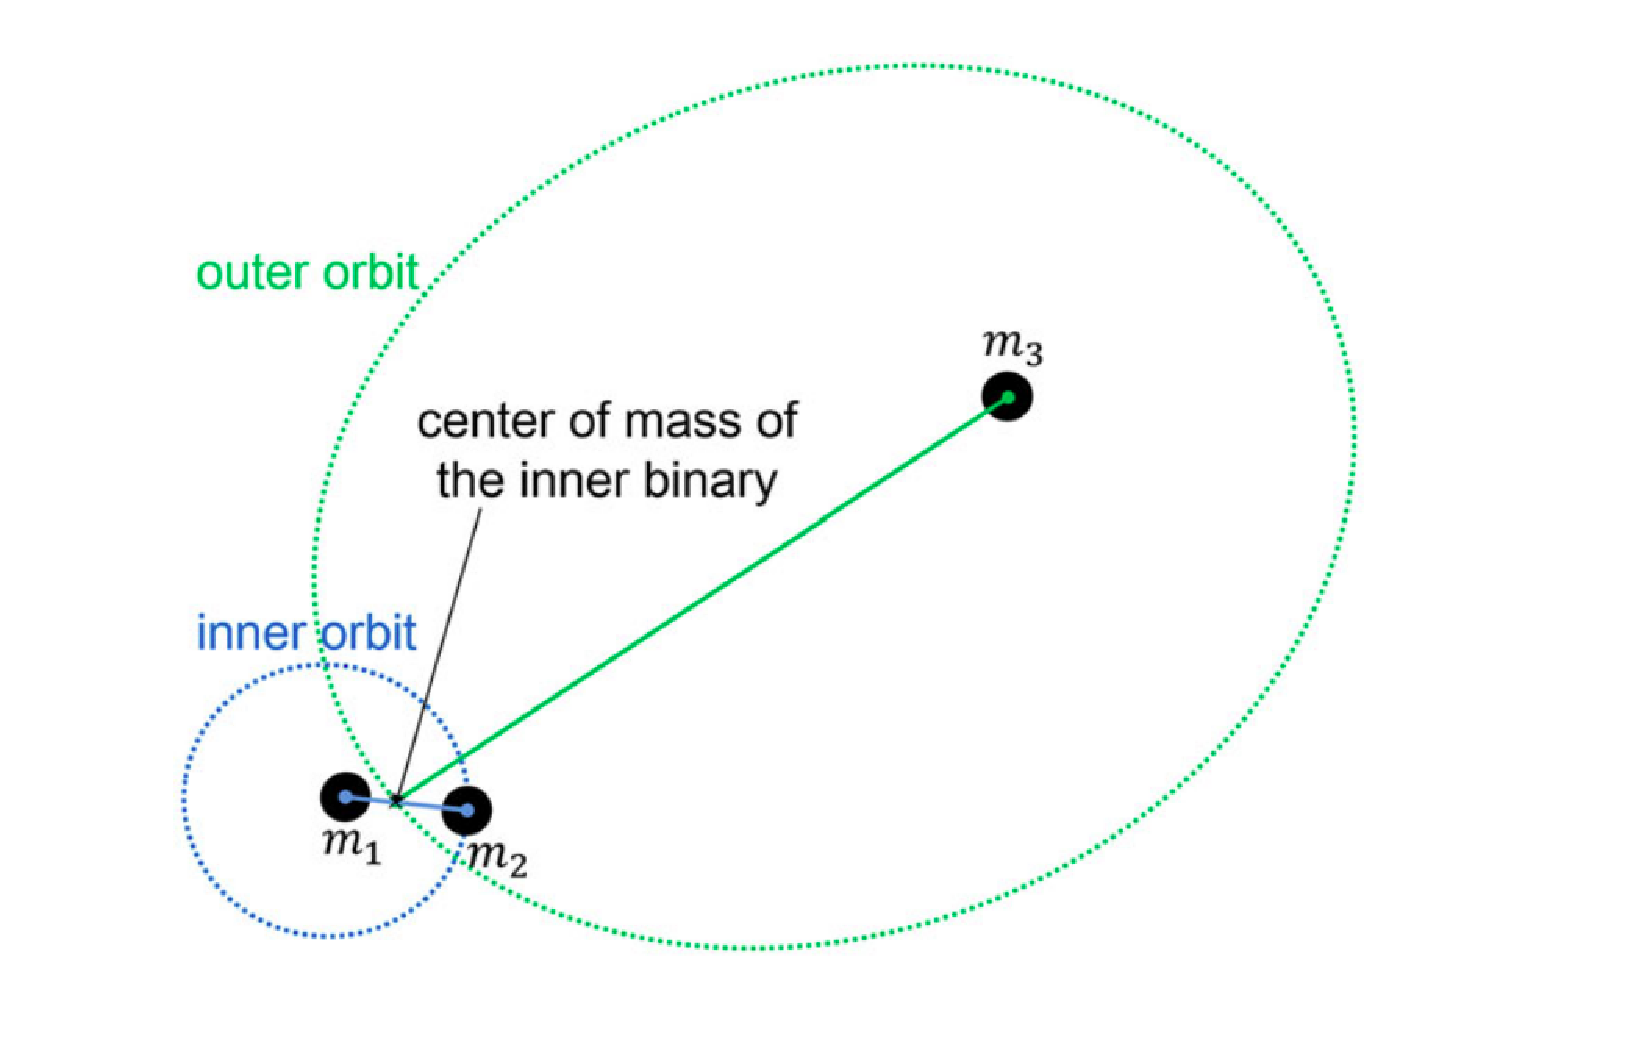
\includegraphics[width=0.9\textwidth]{Thesis/figures/triple_schem.pdf}
    \caption{A schematic of a hierarchical triple system consisting of an inner and an outer binary. The inner binary consists of objects whose masses are $m_1$ and $m_2$, and the outer one is the pair of the inner binary and the third body with mass $m_3$. Figure taken by \cite{gupta2020gravitational}.}
    \label{fig:triple_schem}
\end{figure}
In certain situations, the presence of the outer star does not alter the evolution of the inner binary. In such cases, the evolution of the tertiary  and the inner binary can be studied separately. In other circumstances, the three stars interact in ways that are unique to systems with multiplicities higher than binaries. As a result, numerous new evolutionary paths are anticipated compared to binary evolution. In the following subections, I focus on the dynamical stability of triple systems and the Lidov-Kozai cycles. These topics are relevant to my work, but for a detailed overview of triple evolution I direct the reader to \cite{michaely2014secular,toonen2016evolution}.

\subsection{Stability of triples}\label{sub:stability_triples}

Unlike two-body systems, the three-body problem does not have closed-form solutions. On the one hand, triple systems in the unstable regime tend to disintegrate into lower order systems on dynamical timescales \citep{van2007formation}. On the other hand, stability can occur (and last) on different timescales, thus it is not trivial to draw a clear line between stable and unstable triple systems. 

\cite{mardling1999dynamics} stability criterion is usually used in studies of triple systems' evolution, where a system is unstable if
$\frac{\alpha_{in}}{\alpha_{out}} < \frac{\alpha_{in}}{\alpha_{out}} |_{crit}$. The critical fraction is given as:
\begin{equation}\label{eq:stability_regime}
    \frac{\alpha_{in}}{\alpha_{out}} |_{crit} = \frac{2.8}{1-e_{out}} (1- \frac{0.3 i_{mut}}{\pi}) \left ( \frac{(1 + q_{out})(1+e_{out})}{\sqrt{1-e_{out}}} \right )^{2/5},
\end{equation}
where $q_{out} \equiv m_3 / (m_1 + m_2)$. The criterion is based on the concept of chaos and the result of overlapping resonances. The criterion is conservative since the existence of chaos is not always synonymous with instability. Many more stability criteria have been proposed and I direct the reader to \cite{mardling2001stability,georgakarakos2008stability}.

In \cref{sub:orbit_evol_mass_loss} I discussed how the orbital parameters change during non-conservative mass transfer. These concepts are also applicable for triples, where the orbital parameters of the inner and the outer orbit can change due to angular momentum loss from the system. As a result, initially stable triple systems can become dynamically unstable during their evolution.

\subsection{Lidov-Kozai cycles}\label{sub:lidov_kozai}

Dynamical interactions in hierarchical triples can differ from the case of binaries. The presence of the third star can give rise to the Lidov-Kozai mechanism \citep{lidov1962evolution,kozai1962secular}, which can have a significant impact on the secular evolution the system. During Lidov-Kozai cycles, the mutual torque between the inner and outer binary orbits result to angular momentum exchange. Furthermore, the orbital energy is preserved, and hence the semi-major axes are also conserved. Consequently, the orbital inner eccentricity and mutual inclination vary periodically (i.e. 'cycles'). When the inclination between the two orbits is minimized, the inner binary's eccentricity reaches its maximum. Furthermore, the pericenter argument may rotate or librate periodically.

Evolution during Lidov-Kozai cycles can be fairly complicated, but given some assumptions, analytical expressions can be derived. For example, in the test-particle approximation ($e_{in}=e_{out}=0$ and $M_2 << M_1, M_3$ \citep{naoz2013secular}), the mechanism is expected to take place only if $i_{mut} \in [39.2^{\circ},140.8^{\circ}$]. Furthermore, by expanding the three-body Hamiltonian to quadrupole order in $a_{in}/a_{out}$ \citep{kinoshita1999analytical}, the timescale for the Lidov-Kozai cycles is
\begin{equation}\label{eq:lidov_kozai_timescale}
    t_{kozai} \approx \frac{P_{out}^2}{P_{in}} + \frac{M_1 + M_2 +M_3}{M_3}(1-e_{out}^2)^{3/2},
\end{equation}
where $P_{in}$ and $P_{out}$ are the periods of the inner and outer orbit, respectively. Typically, $t_{kozai} >> P_{in},P_{out}$.

Higher orders of $a_{in}/a_{out}$, i.e. the octupole level of approximation, result to even richer dynamical behavior than the quadrupole approximation. The octupole term is expected to be important when $\epsilon_{oct} \geq 0.01$ \citep{naoz2011hot,shappee2013mass} and
\begin{equation}\label{eq:octupole_term}
    \epsilon_{oct} = \frac{M_1 - M_2}{M_1 + M_2} \frac{a_{in}}{a_{out}} \frac{e_{out}}{1-e_{out}^2}.
\end{equation}

\section{Scientific Codes}\label{sec:scientific_codes}

In this section, I introduce the scientific codes that I coupled together in order to simulate the evolution of my target system.  Because these codes can be used in a variety of astrophysical scenarios, I will concentrate on their fundamental usage and working principles. I encourage users who want to dig deeper into the codes to follow the relevant citations. 

\subsection{MESA}

MESA (Modules for Experiments in Stellar Astrophysics, \cite{paxton2010modules,paxton2013modules,paxton2015modules,paxton2019modules}) is a powerful and versatile 1D stellar evolution code that has become one of the most widely used tools in modern astrophysics. The code is written in Fortran and is designed to solve the fully coupled structure and composition equations simultaneously, allowing for highly accurate models of stars.

MESA includes a wide range of physics modules for various astrophysical processes, such as the equation of state, nuclear reaction networks, hydrodynamics, convective and radiative energy transport, mass loss, rotation, and magnetic fields. The code can simulate the evolution of stars from their birth to their death, including complex phases such as helium and carbon burning, thermal pulses, and supernova explosions. As a result, MESA is an invaluable tool for astrophysical research, from studying the formation and evolution of stars to exploring the origins of the elements in the universe.

The central feature of MESA is the solution of the coupled structure and composition equations, which describe the internal structure of stars and the evolution of their chemical composition over time. These equations are based on fundamental principles of stellar physics, such as conservation of mass, momentum, and energy, as well as nuclear reactions that generate and consume energy in the star. The structure and composition equations can be written as a set of coupled differential equations that describe the evolution of the mass, radius, luminosity, temperature, and chemical composition of the star over time \citep{paxton2010modules,paxton2013modules,paxton2015modules,paxton2019modules}).

MESA also includes a comprehensive nuclear reaction network that describes the fusion of light elements into heavier elements in the stellar core. The network includes thousands of nuclear reactions that involve hundreds of isotopes, making it one of the most detailed and accurate nuclear reaction networks available for stellar evolution calculations.


\subsection{GADGET-2}\label{sub:gadget2}

A detailed documentation of GADGET-2 is out of the scope of this section. Nevertheless, GADGET-2, is the main code used in my simulations, thus the general description of the code will be followed by the basic principles behind the calculation of hydro- and collisionless dynamics.

GADGET-2 (GAlaxies with Dark matter and Gas intEracT) is a smoothed particle hydrodynamics (SPH) code that simulates the gravitational and hydrodynamic evolution of collisionless and gaseous systems in astrophysical contexts \citep{springel2005cosmological}. The code is capable of modeling a wide range of physical processes, such as gas dynamics, gravity, magnetic fields, and radiative transfer. GADGET-2 is written in C++ and is publicly available under the GNU General Public License.

The hydrodynamics computation in GADGET-2 is performed by solving the equations of motion for each particle in the simulation domain. The acceleration of each particle is calculated by summing the forces acting on it, including gravity, pressure gradients, and artificial viscosity. The gravity calculation uses the hybrid TreePM method \citep{bode2000tree,bagla2002treepm}, where the simulation volume is recursively subdivided into cubic cells, with each cell containing a maximum number of particles. The algorithm then builds a tree structure where each cell is treated as a node, and nodes that are spatially close are grouped together to form larger nodes. The final tree structure is used to compute the gravitational force on each particle avoiding the need to calculate the force between all pairs of particles in the system. This method reduces the computational cost from $O(N^2)$ for direct summation to $O(N\log N)$, where $N$ is the number of particles.

The code also includes modules for modeling magnetic fields and radiative transfer. The magnetic field module includes algorithms for calculating the magnetic field evolution and its effects on the gas dynamics. The radiative transfer module includes algorithms for calculating the transport of radiation through the simulation domain and its effects on the gas and dust properties. GADGET-2 can be run in parallel on high-performance computing clusters using the Message Passing Interface (MPI) standard.

\subsubsection{Hydrodynamics}

The basic principle of the SPH method is that the fluid is represented as a set of particles with associated physical attributes such as density, pressure, and velocity. These properties are calculated at a given point in space, using the interpolation method. The method allows any function to be defined in terms of its values at a group of disordered points known as particles \citep{monaghan1982particle}. The integral interpolant of any function $f(r)$ is defined by:
\begin{equation}\label{eq:interpolant}
    \langle f(r) \rangle = \int f(r') W(r-r',h) dr'
\end{equation}
where the integration is performed across the entire space and $W$ is an interpolating/smoothing kernel. Furthermore, the method is Lagrangian, meaning that the particles move with the fluid and do not have a fixed position in space.

The smoothing kernel has two basic properties, similar with Dirac's delta function:
\begin{equation}\label{eq:kernel_property_1}
    \int W(r-r',h) dr' = 1
\end{equation}
and
\begin{equation}\label{eq:kernel_property_2}
   \lim_{h\to0} W(r-r',h) = \delta(r-r').
\end{equation}

GADGET-2 code uses the cubic spline kernel of \cite{monaghan1985refined}:
\begin{equation}\label{eq:spline_kernel}
  W(|r|,h) = \frac{1}{\pi h^3}
    \begin{cases}
      1 - \frac{3}{2}q^2 + \frac{3}{4}q^3, & 0 \leq q < 1\\
      \frac{1}{4}(2 - q)^3, & 1 \leq q <2 \\
      0, &  q \geq 2,
    \end{cases}      
\end{equation}
where $q = \frac{r}{h}$. The kernel is smooth and has a compact support, meaning it averages the properties of neighboring particles within a certain radius, called smoothing length, $h$, of the target point.  

When $q \geq 2$, there is no interaction, since $W(|r|,h)$ is zero. Thus, the amount of interactions for each particle is determined by the smoothing length $h$. When $h$ is too small, there aren't enough particles to interact with, resulting in poor precision. When $h$ is too large, local characteristics are scattered out too much, resulting in low precision and sluggish computation. Hence, the selection of the smoothing kernel, as well as an appropriate smoothing duration, is critical for both accuracy and speed. 

To make the most of SPH's Lagrangian nature, one must accommodate for an adaptive $h$. The smoothing length should be small in high-density regions and large in low-density regions. For example, the density estimate,  which GADGET-2 does is in the form of:
\begin{equation}
    \rho_i = \sum_{j=1}^{N} m_j W(r_i -r_j,h_i),
\end{equation}
where adaptive smoothing lengths $h_i$ of each particle are designed in such a way that their kernel volumes contain a constant mass for the estimated density, implying that the smoothing lengths and estimated densities follow the (implicit) equations
\begin{equation}
    \frac{4\pi}{3} h_{i}^3 \rho_i = N_{sph} \bar{m}
\end{equation}
where $N_{sph}$ is the typical number of smoothing neighbours, and $\bar{m}$ is an average particle mass. In my simulations, I use the default value $N_{sph}=50$. 

\begin{comment}
When two gas particles approach each other the contribution of viscosity in their equation of motion cannot be ignored. Viscosity results to the transfer of momentum along velocity gradients by random motions of
the gas. To account for that, GADGET-2 (and SPH codes in general) adopts an artificial viscosity scheme.
\end{comment}


\subsubsection{Collisionless dynamics}

In self-gravitating SPH codes such as GADGET-2, the point particles represent a large amount of mass and may get arbitrarily and abnormally near in a simulation, and numerical rounding may blow up. In order to avoid particles from scattering too strongly off of one another on close approach, a softening kernel, is used to also soften gravitational forces. 

\begin{figure}[H]
    \centering
    \includegraphics[width=0.9\textwidth]{Thesis/figures/smoothening.pdf}
    \caption{The functional form of the modified potential (-), gravitational force and the density profile using the cubic spline kernel. Figure taken by \cite{price2007energy}.}
    \label{fig:smoothened_gravity}
\end{figure}

GADGET-2 employs once again the cubic spline kernel, Eq. \eqref{eq:spline_kernel}, where now $h$ refers to the softening lenght. In general the softening length can differ from the smoothing length used in the hydrodynamic calculations, but in my simulations they are equal. The basis for this is \cite{bate1997resolution} study, which demonstrated that in self-gravitating SPH simulations, employing a softening length that differs from the smoothing length might lead in unphysical results. Hence, the modified gravitational potential per unit mass is given as:
\begin{equation}\label{eq:softened_gravity}
   \Phi(r) = -G\sum_{i=1}^{N} m_i W(r-r_i,h)
\end{equation}


The functional form of the modified potential, gravitational force and the density profile using the cubic spline kernel is depicted in \cref{fig:smoothened_gravity}. It is apparent that, for $q \geq 2$, the softening is zero and the potential follows the exact form, $\Phi(r) \propto -\frac{1}{r}$. 

\subsection{Huayno}\label{sub:huayano}

Huayno \citep{pelupessy2012n} is a high-performance N-body integrator code designed to simulate the dynamics of collisionless systems, such as galaxies, star clusters, and dark matter halos. The code is written in C++ and the basic principle of Huayno is the use of a hybrid algorithm \citep{bode2000tree} that combines the particle-mesh (PM) \citep{klypin1983three} and tree-based algorithms \citep{barnes1986hierarchical,dehnen2000very} to reduce the computational cost of simulating large systems.


The PM algorithm represents the gravitational potential as a discrete mesh of fixed resolution, and the particle positions are interpolated onto the mesh using a cloud-in-cell (CIC) scheme. The gravitational forces are then calculated by solving Poisson's equation on the mesh. The tree-based algorithm, on the other hand, uses a hierarchical structure to group particles into clusters and calculates the forces between clusters at different levels of the hierarchy. By combining the advantages of both algorithms, Huayno can handle a wide range of particle distributions and non-equilibrium systems, such as systems with binary or multiple stars.




